\documentclass{beamer}
\usetheme{Berlin}

\usepackage[spanish]{babel}
\usepackage[utf8]{inputenc}
\usepackage[T1]{fontenc}
\usepackage{hyperref}
\usepackage{graphicx}
\usepackage{listings} % Paquete para incluir código fuente

% Configuración del paquete listings para C
\lstdefinestyle{mystyle}{
    backgroundcolor=\color{white},     % Color de fondo
    commentstyle=\color{green},        % Estilo de comentarios
    keywordstyle=\color{blue},         % Estilo de palabras clave
    numberstyle=\tiny\color{gray},     % Estilo de números de línea
    stringstyle=\color{red},           % Estilo de cadenas
    basicstyle=\ttfamily\footnotesize, % Estilo de texto básico
    breakatwhitespace=false,           % Rompe líneas en espacios
    breaklines=true,                   % Rompe líneas largas
    numbers=left,                      % Números de línea a la izquierda
    numbersep=5pt,                     % Separación de números de línea
    showspaces=false,                  % No muestra espacios
    showstringspaces=false,            % No muestra espacios en cadenas
    tabsize=2,                         % Tamaño de tabulación
}

\lstset{style=mystyle} % Aplica el estilo definido

\title{Bootloaders}
\subtitle{Teoría e implementación}
\author{Mg. Ing. Gonzalo Nahuel Vaca}
\institute{AADECA}
\date{14 de noviembre de 2024} % Fecha fija de la presentación

% Configuración para que las portadas de sección estén en español
\addto\captionsspanish{
  \renewcommand{\contentsname}{Contenido}
  \renewcommand{\partname}{Parte}
  \renewcommand{\appendixname}{Apéndice}
  \renewcommand{\figurename}{Figura}
  \renewcommand{\tablename}{Tabla}
}

% Personalización de \sectionpage en español
\setbeamertemplate{section page}{
    \begin{centering}
        \begin{beamercolorbox}[sep=12pt,center]{part title}
            \usebeamerfont{section title}\insertsection\par
        \end{beamercolorbox}
    \end{centering}
}

\begin{document}

% Portada
\begin{frame}
    \titlepage
\end{frame}

% Tabla de Contenidos
\begin{frame}{Contenido}
    \tableofcontents
\end{frame}

% Sección 1
\section{Introducción}
\begin{frame}
    \sectionpage % Genera la portada de la sección
\end{frame}

\begin{frame}{¿Qué es un bootloader?}
    \begin{block}{BOOT - Momento de ejecución}
        \emph{ARRANQUE}
    \end{block}
    \begin{block}{LOADER - Funcionalidad}
        \emph{CARGA OTRO PROGRAMA}
    \end{block}
\end{frame}

\begin{frame}{¿Para que sirve un bootloader?}
    \begin{block}{Root of Trust}
        Punto de confianza inicial en un esquema de ciberseguridad.
    \end{block}
    \begin{block}{Verificar integridad}
        Puede validar la firma del programa a ejecutar.
    \end{block}
    \begin{block}{Actualizaciones}
        Ofrece \emph{Serial Recovery} y permite actualizaciones \emph{Over The Air}
    \end{block}
\end{frame}

% Sección 2
\section{Teoría de funcionamiento}
\begin{frame}
    \sectionpage % Genera la portada de la sección
\end{frame}

\begin{frame}{Funcionamiento básico}
    \centering
    \includegraphics[width=1\textwidth]{img/bootloader001.pdf}
\end{frame}

\begin{frame}{Root of Trust}
    \centering
    \includegraphics[width=0.7\textwidth]{img/bootloader002.pdf}
\end{frame}

\begin{frame}{Serial Recovery}
    \centering
    \includegraphics[width=1\textwidth]{img/bootloader003.pdf}
\end{frame}

\begin{frame}{Firmware Over The Air (FOTA) Update}
    \centering
    \includegraphics[width=0.65\textwidth]{img/bootloader004.pdf}
\end{frame}

% Sección 3
\section{Implementación}
\begin{frame}
    \sectionpage % Genera la portada de la sección
\end{frame}

\begin{frame}{Arquitectura}
    \begin{alertblock}{Aclaración}
        Implementación válida para microcontroladores ARM Cortex M.
    \end{alertblock}
\end{frame}

\begin{frame}{Modelo de memoria}
    \centering
    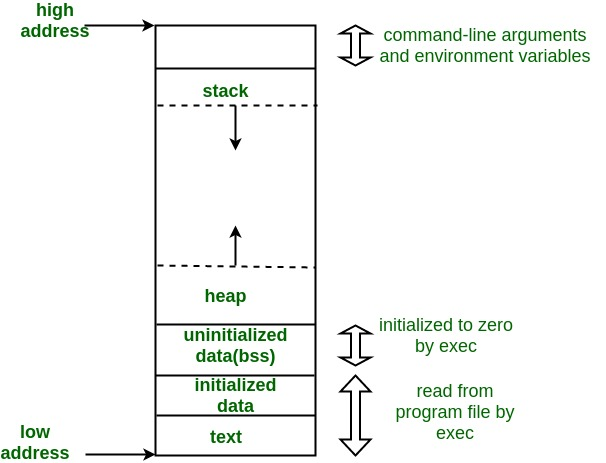
\includegraphics[width=0.8\textwidth]{img/memory.jpg}
\end{frame}

\begin{frame}{Vector Table Offset Register}
    \centering
    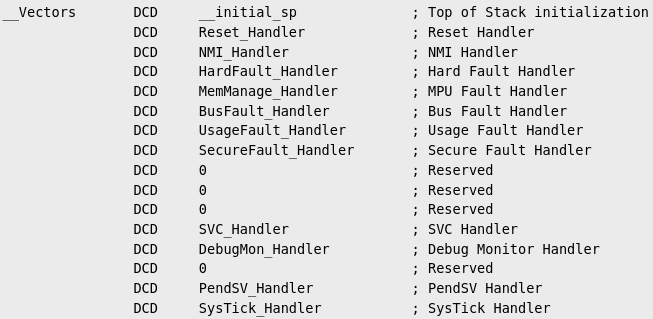
\includegraphics[width=1\textwidth]{img/vector_table.png}
\end{frame}

% Ejemplo de inclusión de código en C
\begin{frame}[fragile]{CMSIS GCC - Start}
    \begin{lstlisting}[language=C]
__STATIC_FORCEINLINE __NO_RETURN void __cmsis_start(void)
{
    extern void _start(void) __NO_RETURN;

    /* ... */

    extern const __copy_table_t __copy_table_start__;
    extern const __copy_table_t __copy_table_end__;
    extern const __zero_table_t __zero_table_start__;
    extern const __zero_table_t __zero_table_end__;

    /* ... */
}
    \end{lstlisting}
\end{frame}

\begin{frame}[fragile]{CMSIS GCC - Atributo VECTOR TABLE}
    \begin{lstlisting}[language=C]
#ifndef __VECTOR_TABLE
#define __VECTOR_TABLE            __Vectors
#endif

#ifndef __VECTOR_TABLE_ATTRIBUTE
#define __VECTOR_TABLE_ATTRIBUTE  __attribute__((used, section(".vectors")))
#endif
    \end{lstlisting}
\end{frame}

\begin{frame}[fragile]{Saltar a la aplicación}
    \begin{lstlisting}[language=C]
#include <stdint.h>
#include "cmsis_gcc.h"

__attribute__((noreturn)) void jump_to_application(uint32_t app_address)
{
    uint32_t msp = *(uint32_t *)(app_address);
    uint32_t reset_vector = *(uint32_t *)(app_address + 4U);
    __set_MSP(msp); // __ASM volatile ("MSR msp, %0" : : "r" (topOfMainStack) : );
    asm volatile("bx %0" : : "r"(reset_vector));
    while(1);
}
    \end{lstlisting}
\end{frame}

\begin{frame}[fragile]{Makefile - Toolchain y Flags}
    \begin{lstlisting}[language=C]
PREFIX ?= arm-none-eabi-

AR      := $(PREFIX)ar
AS      := $(PREFIX)as
CC      := $(PREFIX)gcc
CXX     := $(PREFIX)g++
GDB     := $(PREFIX)gdb
LD      := $(PREFIX)gcc
OBJCOPY := $(PREFIX)objcopy
OBJDUMP := $(PREFIX)objdump

CFLAGS = -mthumb -mcpu=cortex-m4
    \end{lstlisting}
\end{frame}

\begin{frame}[fragile]{Makefile - Targets}
    \begin{lstlisting}[language=C]
snipets.objdump: snipets.o
    @$(OBJDUMP) -d $< > $@

snipets.o: snipets.c
    $(CC) $(CFLAGS) -c $< -o $@

clean:
    -rm snipets.o snipets.objdump

.PHONY: clean
    \end{lstlisting}
\end{frame}

% Sección 4
\section{Tecnologías disponibles y uso real}
\begin{frame}
    \sectionpage % Genera la portada de la sección
\end{frame}

\begin{frame}{Zephyr RTOS + MCUboot}
    \centering
    
\includegraphics[width=0.8\textwidth]{img/zephyr.png}
\end{frame}

\begin{frame}{Eclipse hawkBit}
    \centering
    
\includegraphics[width=0.8\textwidth]{img/hawkbit.png}
\end{frame}

\begin{frame}{Ejemplo real: Pump Control}
    \begin{block}{Desafíos}
        \begin{itemize}
            \item Disperción geográfica (Egipto, India, LATAM, etc.).
            \item Robo de propiedad intelectual.
            \item Sistemas críticos.
        \end{itemize}
    \end{block}
    \begin{block}{Soluciones}
        \begin{itemize}
            \item Bootloaders propios.
            \item Programadores de producción y de \emph{calle}.
            \item Sistema de gestión y despliegue de firmware propio.
        \end{itemize}
    \end{block}
\end{frame}



% Frame de agradecimiento fuera de cualquier sección
\appendix
\begin{frame}
    \centering
    \Huge Gracias por su atención
    \vfill
    % Añade el correo electrónico y LinkedIn
    \normalsize
    \textbf{Contacto:} \href{mailto:vacagonzalo@gmail.com}{vacagonzalo@gmail.com} \\
    \textbf{LinkedIn:} \href{https://www.linkedin.com/in/vaca-gonzalo}{linkedin.com/in/vaca-gonzalo} \\
    \textbf{Github:} \href{https://github.com/vacagonzalo/aadeca-bootloaders-2024}{github.com/vacagonzalo/aadeca-bootloaders-2024}
\end{frame}

\end{document}
